\documentclass[UTF8]{ctexart}

%固定图片位置
\usepackage{float}

%插入超链接
\usepackage{url}

\usepackage{tikz,mathpazo}
\usetikzlibrary{shapes.geometric, arrows}
\usetikzlibrary{calc}

%\usepackage[affil-it]{authblk}

\usepackage{listings}
%插入代码的配置
\definecolor{CPPLight}  {HTML} {686868}
\definecolor{CPPSteel}  {HTML} {888888}
\definecolor{CPPDark}   {HTML} {262626}
\definecolor{CPPBlue}   {HTML} {4172A3}
\definecolor{CPPGreen}  {HTML} {487818}
\definecolor{CPPBrown}  {HTML} {A07040}
\definecolor{CPPRed}    {HTML} {AD4D3A}
\definecolor{CPPViolet} {HTML} {7040A0}
\definecolor{CPPGray}  {HTML} {B8B8B8}
\lstset{
	language=Matlab,                                     % 设置语言
    columns=fixed,    
    breaklines = true,   
    basicstyle=\small ,
    numbers=left,                                        % 在左侧显示行号
    %frame=none,                                          % 不显示背景边框
    backgroundcolor=\color[RGB]{245,245,244},            % 设定背景颜色
    keywordstyle=\color[RGB]{40,40,255}\bfseries,                 % 设定关键字颜色
    %commentstyle=\color{red!10!green!70}\textit,    % 设置代码注释的颜色
    numberstyle=\tiny\color{darkgray},           % 设定行号格式
    commentstyle=\it\color[RGB]{0,96,96},                % 设置代码注释的格式
    stringstyle=\rmfamily\slshape\color[RGB]{128,0,0},   % 设置字符串格式
    showstringspaces=false,                              % 不显示字符串中的空格                           
    %morekeywords={True,alignas,continute,friend,register,true,alignof,decltype,goto,
    %reinterpret_cast,try,asm,defult,if,return,typedef,auto,delete,inline,short,
    %typeid,bool,do,int,signed,typename,break,double,long,sizeof,union,case,
    %dynamic_cast,mutable,static,unsigned,catch,else,namespace,static_assert,using,
    %char,enum,new,static_cast,virtual,char16_t,char32_t,explict,noexcept,struct,
    %void,export,nullptr,switch,volatile,class,extern,operator,template,wchar_t,
    %const,false,private,this,while,constexpr,float,protected,thread_local,
    %const_cast,for,public,throw,std,rand},
    emph={access,and,break,class,continue,def,del,elif ,else,%
	except,exec,finally,for,from,global,if,import,in,i s,%
	lambda,not,or,pass,print,raise,return,try,while, imshow, subplot, figure,%
    log, fft2, fftshift, abs, size, rgb2gray, imread},
    emphstyle=\color{CPPViolet}\bfseries, 
    emph={[2]True, False, None, self},
	emphstyle=[2]\color{green},
	emph={[3]from, import, as},
	emphstyle=[3]\color{blue},
	upquote=true,
	morecomment=[s]{"""}{"""},
    morecomment=[s]{\%}{},
	%commentstyle=\color{orange}\slshape,
    commentstyle=\color{red!10!green!70}\textit,    % 设置代码注释的颜色
	emph={[4]1, 2, 3, 4, 5, 6, 7, 8, 9, 0},
	emphstyle=[4]\color{red},
	emph={[5]numpy, np, plt},
	emphstyle=[5]\color{red},
	literate=*{:}{{\textcolor{blue}:}}{1}%
	{=}{{\textcolor{blue}=}}{1}%
	{-}{{\textcolor{blue}-}}{1}%
	{+}{{\textcolor{blue}+}}{1}%
	{*}{{\textcolor{blue}*}}{1}%
	{!}{{\textcolor{blue}!}}{1}%
	{(}{{\textcolor{blue}(}}{1}%
	{)}{{\textcolor{blue})}}{1}%
	{[}{{\textcolor{blue}[}}{1}%
	{]}{{\textcolor{blue}]}}{1}%
	{<}{{\textcolor{blue}<}}{1}%
	{>}{{\textcolor{blue}>}}{1},%
    %{\%}{{\textcolor{green}\%}}{1},%
	framexleftmargin=0.1mm, framextopmargin=0.1mm, frame=shadowbox, rulesepcolor=\color{black},
}



\usepackage{geometry}
\geometry{left=2cm, right=2cm, top=1.2cm, bottom=1.2cm}

%得到引用的标题内容
\usepackage{nameref} 

%添加首行缩进,两个字符
\usepackage{indentfirst}
\setlength{\parindent}{2em}

%多行公式一个编号
\usepackage{amsmath}

%文献引用,标准类型为plain
%\usepackage[hyperref=true,backend=biber,sorting=none,backref=true]{biblatex}
%\addbibresource{ref.bib}
\bibliographystyle{plain}
\usepackage{cite}

\pagestyle{plain}

%跨页表格
\usepackage{multirow}
\usepackage{longtable,booktabs}
\usepackage{supertabular}
\usepackage{makecell}

%调整itemize等的间距
\usepackage{enumitem}


\usepackage{graphicx}
\usepackage{subfigure}

%超链接
\usepackage[linkcolor=yellow,citecolor=red,backref=page,hyperfootnotes=true]{hyperref}
\hypersetup{
bookmarks=true,
colorlinks=true,
linkcolor=black
}
\usepackage{tabularx} %This package must be placed after package {hyperref}, otherwise footnote marks are NOT treated as hyperlinks.


%引入了一些改进的数学环境,如align
\usepackage{amsmath}

\title{数字图像处理报告十:灰度图像形态学处理}
\author{姓名:鲁国锐 \protect\newline
\and 学号:17020021031 \\
\and 专业:电子信息科学与技术}


\begin{document}
	\maketitle
	\renewcommand{\contentsname}{目录}
	\renewcommand{\listfigurename}{插图目录}
	\renewcommand{\listtablename}{表格目录}
	\renewcommand{\refname}{参考文献}
	\renewcommand{\abstractname}{摘要}
	\renewcommand{\indexname}{索引}
	\renewcommand{\tablename}{表}
	\renewcommand{\figurename}{图}
	
	
	
	\tableofcontents
	\newpage
	
	\hypersetup{
	bookmarks=true,
	colorlinks=true,
	linkcolor=red,
	urlcolor=blue
	}
    
    
	\section{题目描述}
	\indent 思考下如何对灰度图像直接做形态学操作(可查阅文献)。

			
    \section{形态学图像处理简述}\label{introduction}
        
        \indent 形态学通常表示生物学的一个分支,该分支主要研究动植物的形态和结构\cite{digit_image_Gonzalez}。在图像处理领域,这一术语表示数学形态学(也称图像代数)。它作为一种数学工具为我们从图像中提取信息提供了有力的支持。其基本思想为“用具有一定形态的结构元素,去量度和提取图像中的对应形状,以达到对图像分析和识别的目的”\cite{zhang2005图像工程}。
        
        \indent 数学形态学的理论基础和语言是集合论。不同于在传统方法中占有重要地位的线性系统理论,数学形态学是一种非线性图像处理和分析理论\cite{冯桂2000灰度图像边缘检测中的形态学方法}。在这门理论中,用集合表示图像中的对象,它既可以是二值图像,也可以是灰度(彩色)图像。这样做的一个自然结果是形态学算子的性能将主要以几何方式进行刻画,而传统的数值建模分析方法则以解析的方式描述算子的性能,而显示的几何描述特点更适合于视觉信息的处理和分析\cite{冯桂2000灰度图像边缘检测中的形态学方法},这也是用数学形态学进行图像处理的一个显著优势。
        
        \indent 对于不同的图像(二值和灰度等),数学形态学的基本运算与算法也不尽相同,但经常用到的都可归结为四类:膨胀、腐蚀、开启和闭合。本次报告将在第\ref{binary}节和\ref{grayscale}节中分别针对二值图像和灰度图像中的形态学操作进行简要介绍。
    
    
    \section{二值图像中的形态学操作}\label{binary}
        
        \indent 本节主要参考:《图像工程》\cite{zhang2005图像工程};上海交通大学顾力栩教授的慕课“\href{https://www.icourse163.org/course/0809SJTU012-1003381021}{数字图像处理}”
        
        
        \indent 二值形态学中的运算对象是两个集合,一般称$A$为图像集合,$B$为结构元素(本身仍是图像集合),数学形态学运算是用$B$对$A$进行操作。每个结构元素有一个原点,它是结构元素参与形态学运算的参考点,但原点并不一定要属于结构元素。本节中将分别对第\ref{introduction}节中提到的四种运算在二值图像中的操作进行介绍。
        
        
            \subsection{二值膨胀}
                \indent 膨胀的算子为$\oplus$,$A$用$B$来膨胀写作$A \oplus B$,定义为  
                    \begin{align}
                        A \oplus B = \left\{ x \mid \left[ \left( \hat{B} \right)_x \cap A  \right] \neq \emptyset \right\}
                    \end{align} 
                    
                    也可写成
                    \begin{align}
                        A \oplus B = \left\{ x \mid \left[ \left( \hat{B} \right)_x \cap A  \right] \subseteq A \right\}
                    \end{align}                        
                    
                \indent 该操作可以看做是将集合$A$中的每一个非零元素,以$B$中每一个非零元素相对于原点的方向和距离,平移相同的长度,然后对包括原集合在内的每一个平移后的几何去并集,即得膨胀后的结果。
                
                \indent 该操作也可以形象地理解为,用结构元素的原点对$A$中每一个$1$“盖章”,盖章后的结果就是膨胀后的结果。
                

                
            \subsection{二值腐蚀}
                
                \indent 腐蚀的算子为$\ominus$,$A$用$B$来腐蚀写作$A \ominus B$,定义为
                    \begin{align}
                        A \ominus B = \left\{ x \mid \left( B \right)_x \subseteq A \right\}
                    \end{align}                      
                    
                \indent 与膨胀相反,腐蚀操作可以看做是将集合$A$中的每一个非零元素,以$B$中每一个非零元素相对于原点的方向和距离,平移相同的长度,然后对包括原集合在内的每一个平移后的几何取交集的结果。
                
                \indent 同样,该操作也可以形象地理解为,将结构元素的原点依次“摁”在$A$中的每一个$1$上,若结构元素能被完全地包含在$A$中,则该点保留,否则置为$0$。
                
            \subsection{二值开启和闭合}
                
                \indent 膨胀和腐蚀并互为逆运算,所以二者级联使用可以得到不同的结果。如果对图像先腐蚀后膨胀,该操作就称为开启;反之,如果对图像先膨胀后腐蚀,该操作就称为闭合。
                
                \subsubsection{二值开启}
                
                    \indent 开启的算子为$\circ$,$A$用$B$来腐蚀写作$A \circ B$,定义为
                        \begin{align}
                            A \circ B = \left( A \ominus B \right) \oplus B
                        \end{align}                
                
                    \indent 开启运算可以把比结构元素小的突刺滤掉,切断细长搭接而起到分离作用。
            
                \subsubsection{二值闭合}
                
                    \indent 闭合的算子为$\bullet$,$A$用$B$来腐蚀写作$A \bullet B$,定义为
                        \begin{align}
                            A \bullet B = \left( A \oplus B \right) \ominus B 
                        \end{align}           
                
                    \indent 闭合运算可以把比结构元素小的缺口或孔填充上,搭接短的间断而起到连同作用。 
                
%    			\begin{enumerate}[leftmargin=50pt]
%    				\item 数据预处理:
%            			\begin{enumerate}[leftmargin=20pt]
%            				\item 区域划分:降低压缩所需的内存资源,在内存充足的情况下可忽略;
%            				\item 降低量级:将样本的范围从$\left[ 0, 2^P-1 \right]$移到$\left[ -2^P, 2^{P-1}-1 \right]$,从而简化对数值溢出问题的处理;
%            				\item 分量变换:在图像有多个分量时,降低分量之间的相关性,提高压缩效率;
%            			\end{enumerate}
%                    \item 离散小波变换($DWT$):进一步降低数据之间的相关性,并可针对不同类型图像的不同区域采用不同的分辨率,以取得更好的压缩比,而且它还可以提供实现无损压缩的机制;
%                    \item 量化;
%                    \item 自适应算术编码(第一层编码)和码流组织(第二层编码);
%    			\end{enumerate}
		

    \section{灰度图像中的形态学操作}\label{grayscale}
        
        \indent 本节主要参考:《图像工程》\cite{zhang2005图像工程};上海交通大学顾力栩教授的慕课“\href{https://www.icourse163.org/course/0809SJTU012-1003381021}{数字图像处理}”。
        
        \indent 灰度数学形态学与二值数学形态学有密切的联系和对应的关系。二值数学形态学基于集合运算,而在灰度数学形态学中,灰度的排序起着类似的作用;二值数学形态学的操作对象是集合,而在灰度数学形态学中的操作对象是图像函数。
        
        \indent 本节中,以$f\left( x, y \right)$表示输入图像,以$b\left( x, y \right)$表示结构元素,它本身也是一副小图像。
        
        \subsection{灰度膨胀}
            
            \subsubsection{简述}

            \indent 与二值膨胀类似,用结构元素$b$对输入图像$f$进行灰度膨胀记为$f \oplus b$,定义为
                        \begin{align}
                            \left( f \oplus b \right)\left( s, t \right) = \max \left\{ f\left( x, y \right) + b\left( s-x, t-y \right)  \mid \left( x, y \right) \in D_f, \left[ \left( s-x \right), \left( t-y \right) \right] \in D_b \right\} 
                        \end{align}       
             
             式中,$D_f$和$D_b$分别是$f$和$b$的定义域。  
             
             \indent 在二值图像中,膨胀是将集合进行平移,然后求并集的操作,而在灰度图像中则将“集合”这一概念替换为了灰度曲线。而膨胀这一操作在灰度图像中就相当于是将整个曲线进行平移,然后在定义域的并集内所有曲线求最大值。   
             
             \subsubsection{计算实例}
             
                \indent 给定一个曲线,其每个位置取值如图\ref{grey_dilation_calculate}中$F$所示:

                			\begin{figure}[H]
                				\centering 
                				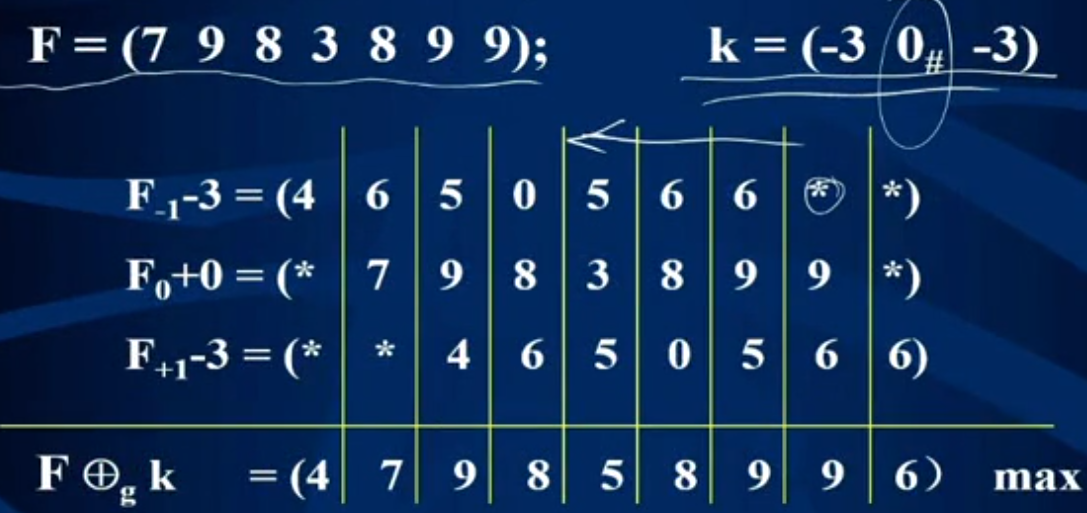
\includegraphics[scale=0.4]{grey_dilation_calculate.png} 
                				\caption{灰度膨胀计算} 
                				\label{grey_dilation_calculate}
                			\end{figure}                 
                            
                \indent 结构元素为$k$,有三个元素,其中$0$是其原点。
                
                \indent 根据膨胀的定义,先将整个曲线沿每一个非零元素相对于原点的方向和距离平移相同的长度,即左右各移动一个单位,如图\ref{grey_dilation_calculate}中$F_{-1}$和$F_{+1}$所示。然后对平移后的曲线加上相应点的值,即左右移动过的曲线各减去$3$,为移动过不变(加$0$)。最后再在这三条曲线中,对每一个位置去最大的值,所得新曲线就是灰度膨胀的结果,如图\ref{grey_dilation_calculate}中$F \oplus _g k$ 所示。
                
                \indent 另外再从几何的层面给出两个二维坐标系中的实例,如图\ref{grey_dilation1}和图\ref{grey_dilation2}所示。
                
                 			\begin{figure}[H]
                 				\centering 
                      			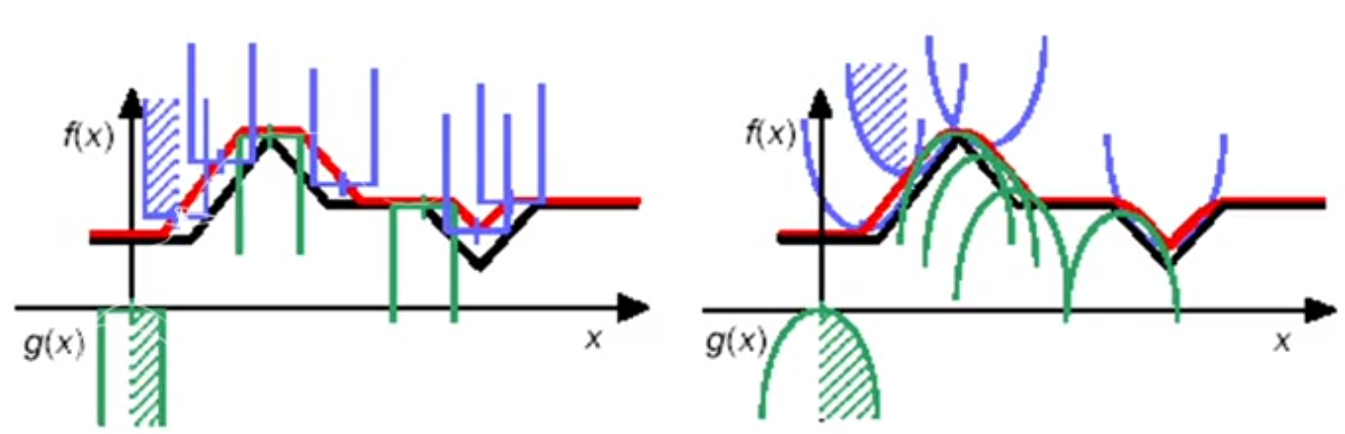
\includegraphics[scale=0.35]{grey_dilation1.png} 
                 				\caption{灰度膨胀实例$1$} 
                 				\label{grey_dilation1}
                 			\end{figure}
             
                 			\begin{figure}[H]
                 				\centering 
                      			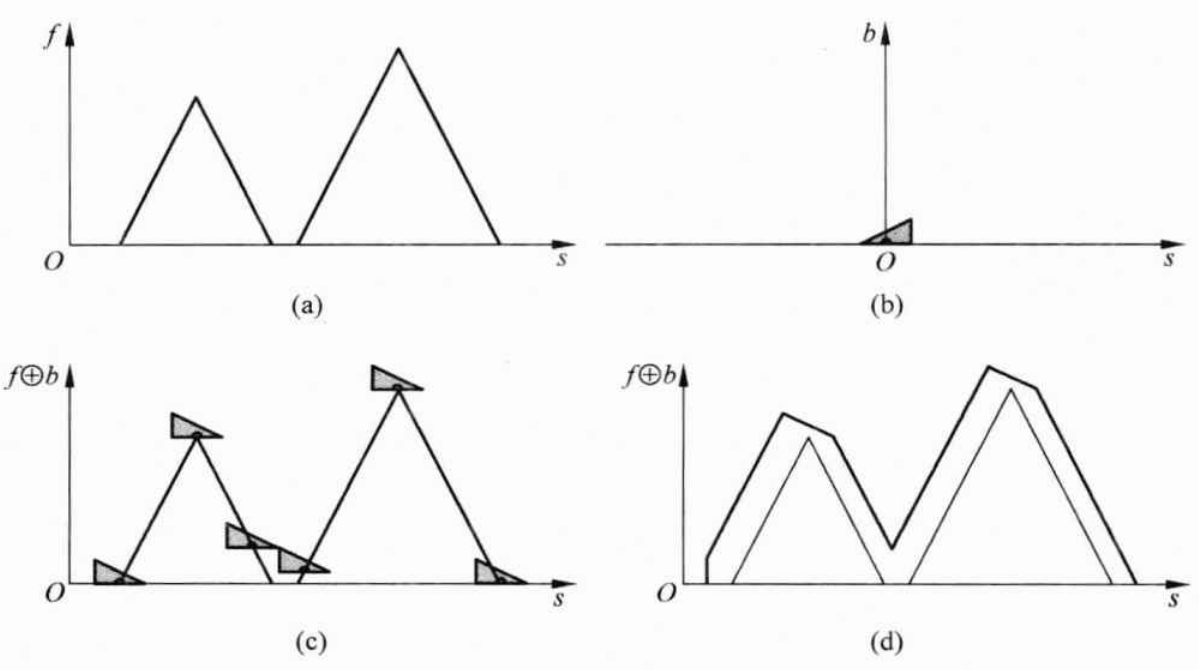
\includegraphics[scale=0.35]{grey_dilation2.png} 
                 				\caption{灰度膨胀实例$2$} 
                 				\label{grey_dilation2}
                 			\end{figure}                             
            
        \subsection{灰度腐蚀}
            
            \subsubsection{简述}
            
            \indent 用结构元素$b$对输入图像$f$进行灰度腐蚀记为$f \ominus b$,定义为
                        \begin{align}
                            \left( f \ominus b \right)\left( s, t \right) = \min \left\{ f\left( x, y \right) - b\left( s+x, t+y \right)  \mid \left( x, y \right) \in D_f, \left[ \left( s+x \right), \left( t+y \right) \right] \in D_b \right\} 
                        \end{align}
                        
            \indent 同二值中的情况类似,灰度腐蚀的操作与灰度膨胀刚好相反:平移方向相反;灰度值做减法;定义域求交集;取最小值。
            
            \subsubsection{计算实例}
            
                \indent 如图\ref{grey_erosion_calculation}所示,给定一条曲线$F$和和结构元素$k$,沿每一个非零元素相对于原点的反方向和距离平移相同的长度,即左右各移动一个单位(注意与图\ref{grey_dilation_calculate}中刚好相反),然后对每条曲线减去结构元素中相应点的值,最后再在这三条曲线定义域的交集中去每一点的最小值,所得新曲线就是灰度腐蚀的结果。

                			\begin{figure}[H]
                				\centering 
                				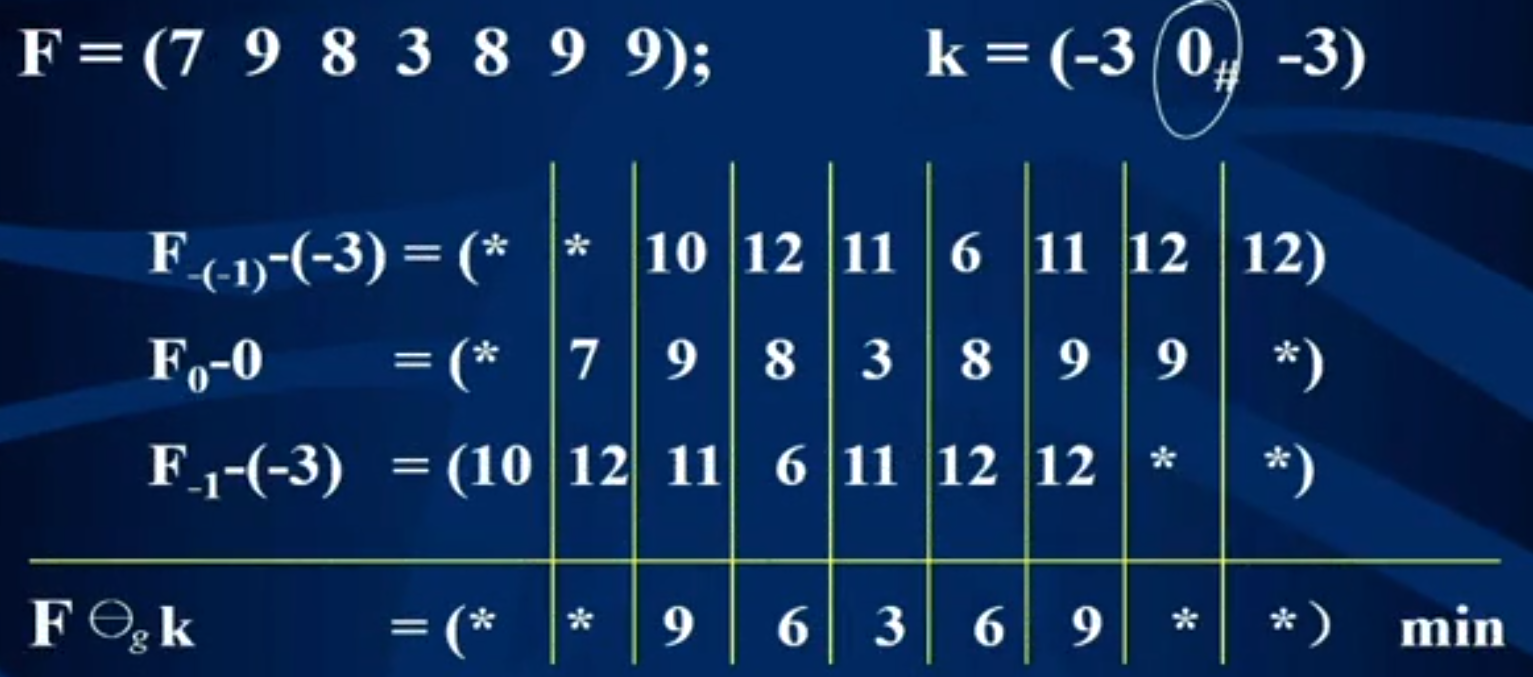
\includegraphics[scale=0.3]{grey_erosion_calculation.png} 
                				\caption{灰度腐蚀计算} 
                				\label{grey_erosion_calculation}
                			\end{figure}                
                
                \indent 本节同样再从几何层面给出两个二维坐标系中的实例,如图\ref{grey_erosion1}和图\ref{grey_erosion2}所示。

                			\begin{figure}[H]
                				\centering 
                				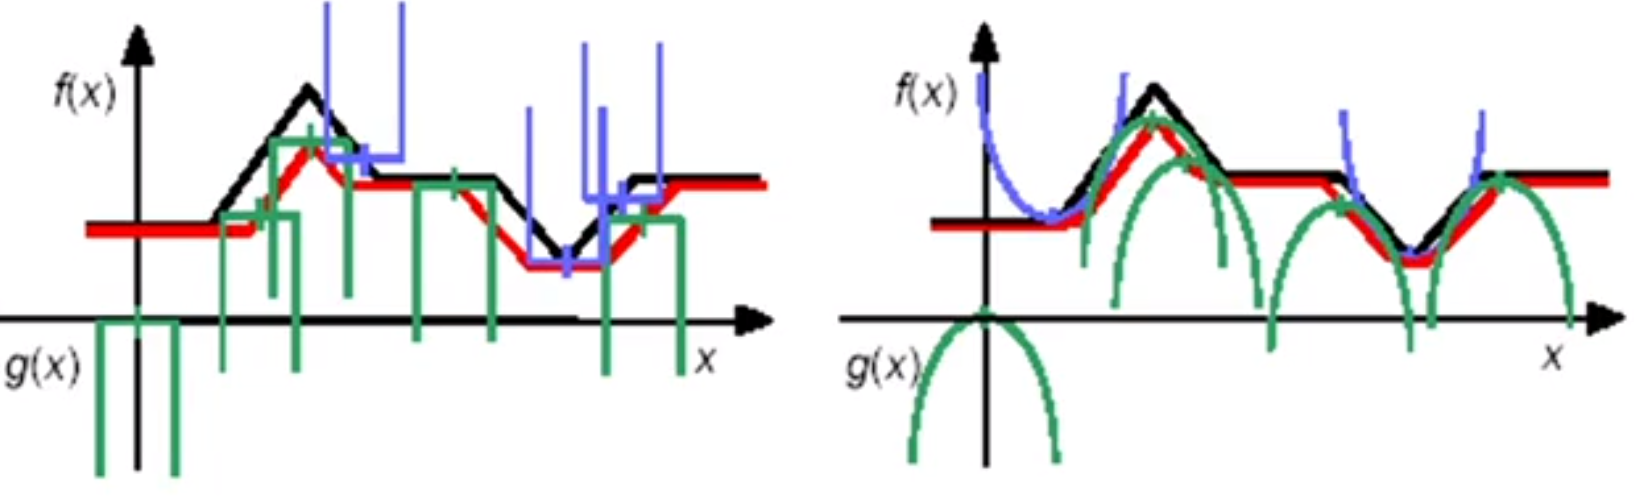
\includegraphics[scale=0.3]{grey_erosion.png} 
                				\caption{灰度腐蚀实例$1$} 
                				\label{grey_erosion1}
                			\end{figure}	


                			\begin{figure}[H]
                				\centering 
                				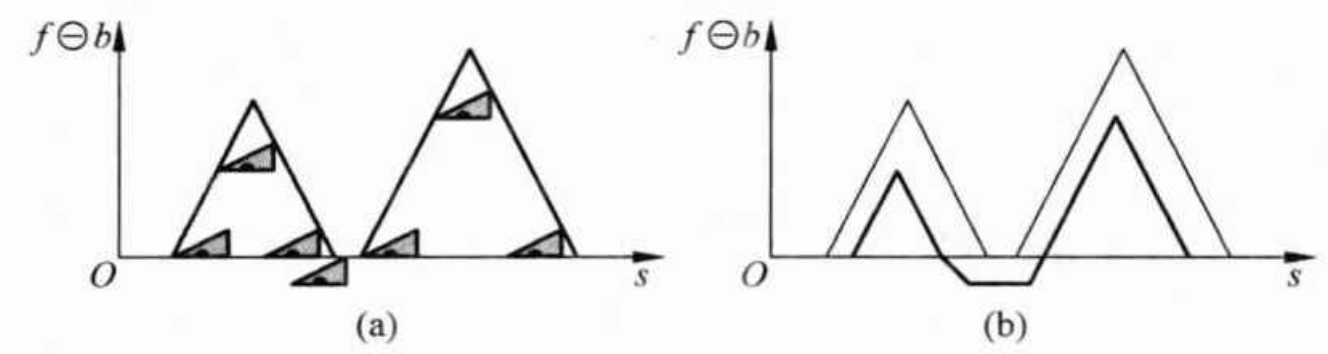
\includegraphics[scale=0.35]{grey_erosion2.png} 
                				\caption{灰度腐蚀实例$2$} 
                				\label{grey_erosion2}
                			\end{figure}     
                            
        \subsection{灰度开启和闭合}
        
            \indent 在灰度图像中,膨胀和腐蚀两个操作仍然不是可逆的。所以与二值的情况类似,通过对这两种操作的排列我们可以得到灰度开启和灰度闭合两种操作。       
            
                \subsubsection{灰度开启}
                
                    \indent 开启的算子为$\circ$,$A$用$B$来腐蚀写作$A \circ B$,定义为
                        \begin{align}
                            A \circ B = \left( A \ominus B \right) \oplus B
                        \end{align}                
                
                    \indent 灰度中的开启运算不仅在尺寸上会去除一些区域,还会将灰度值的“尖峰”抹去或变平滑,如图\ref{grey_opening}所示。

                			\begin{figure}[H]
                				\centering 
                				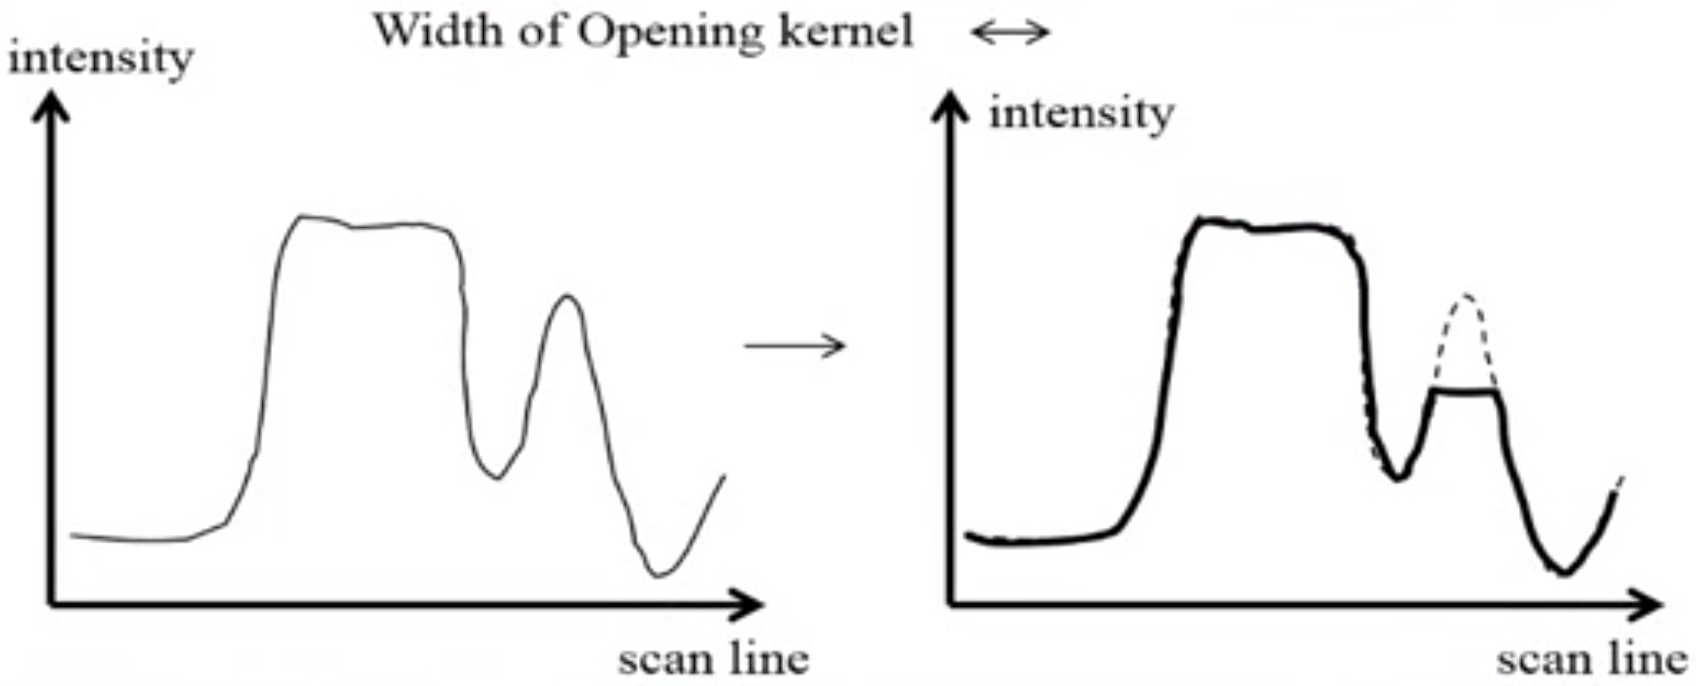
\includegraphics[scale=0.3]{grey_opening.png} 
                				\caption{灰度开启} 
                				\label{grey_opening}
                			\end{figure}
                            
                    \indent 总体而言,开启操作可以概括为:第一步的腐蚀去除了小的亮细节并减弱了图像的亮度,第二步的膨胀基本恢复了图像亮度但又不重新引入之前抹去的亮细节。
                                        
                \subsubsection{灰度闭合}
                
                    \indent 闭合的算子为$\bullet$,$A$用$B$来腐蚀写作$A \bullet B$,定义为
                        \begin{align}
                            A \bullet B = \left( A \oplus B \right) \ominus B 
                        \end{align}           
                
                    \indent 与开启运算相反,闭合运算会将灰度的“尖谷”抹平或变平滑,如图\ref{grey_closing}所示。
                    
                			\begin{figure}[H]
                				\centering 
                				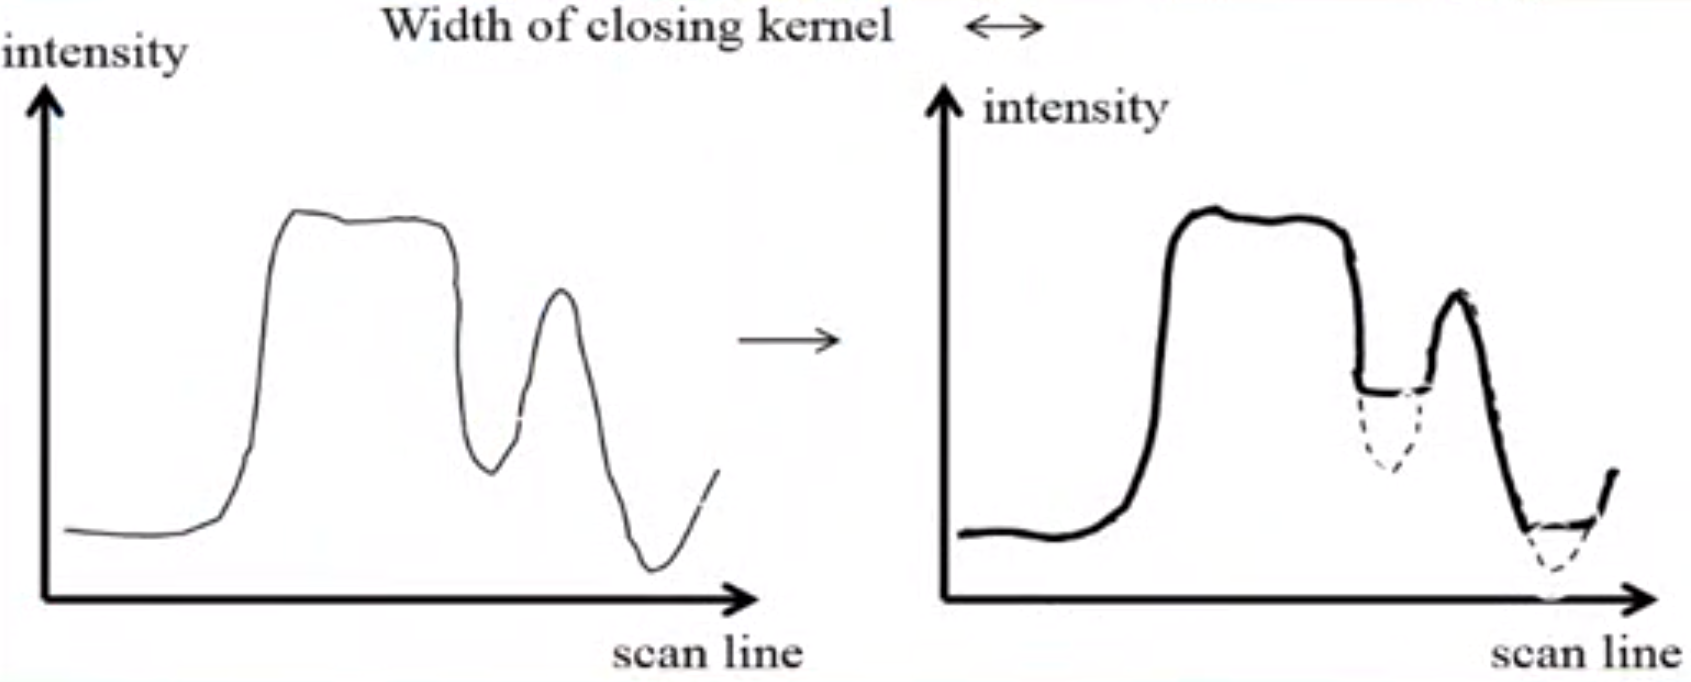
\includegraphics[scale=0.3]{grey_closing.png} 
                				\caption{灰度闭合} 
                				\label{grey_closing}
                			\end{figure}                    
                            
                    \indent 总体而言,闭合操作可以概括为:第一步的膨胀去除了小的暗细节并增强了图像的亮度,第二步的腐蚀基本恢复了图像亮度但又不重新引入之前抹去的暗细节。
                                                      
%	\section{问题背景\protect\footnotemark[1]}\label{background}
%    
%    \footnotetext[1]{本节的写作参考及图像来源:\par 
%            \url{https://www.zhihu.com/question/22864189/answer/40772083} \par
%            \url{http://users.rowan.edu/~polikar/WTtutorial.html}}

%			\begin{figure}[H]
%				\centering 
%				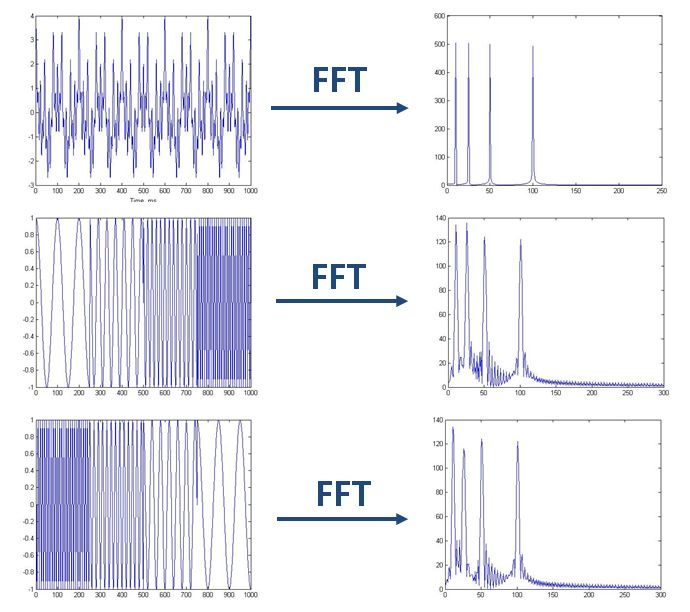
\includegraphics[scale=0.6]{non-stationary.jpg} 
%				\caption{平稳信号和非平稳信号及其傅里叶变换幅频特性} 
%				\label{stationary and non-stationary}
%			\end{figure}                
            

           
            
 
 

        
% 
%                \begin{enumerate}[leftmargin=50pt]
%    				\item 输入一张低分辨率图像,得到其一组特征映射($feature\ maps$);
%    				\item 将得到的特征映射输入到一组子网中,用于预测出高分辨率图像的小波系数;
%    				\item 根据得到的小波系数重建出高分辨率图像。
%    			\end{enumerate}
                

            

  
            
%        \nocite{digit_image_Gonzalez}
%        \nocite{signal_and_system}
%        \nocite{discrete-time_signal_processing}



		

            


%			\indent 采取\ref{数字相机成像原理}节的方式,我们也可以把线性扫描相机的原理概括为以下$3$个步骤:
%			\begin{enumerate}[leftmargin=50pt]
%				\item 由条带传感器成像,给出一幅图像一行(或一列)的像素值;
%				\item 沿垂直于传感器带的方向移动一小段距离;
%				\item 重复步骤$1$和步骤$2$,直至整幅图像全部成像完毕。
%			\end{enumerate}

%		\begin{enumerate}[leftmargin=50pt]
%			\item 所成图像在垂直方向上的大小不受限制;
%			\item 能够通过提高扫描频率达到非常高的分辨率;
%			\item 使用起来灵活方便等
%		\end{enumerate}
		
%	\section{实验验证}
%        \subsection{实验思想}
%            \indent 从前面的分析可以看出,频谱图上的谱线与空间域中像素变化的方向及剧烈程度有关。从这个角度出发,如果把空间域图像转一个角度,频谱图中的谱线相应地也应该旋转相同的角度。我们将在之后的两个小节中对这个猜想进行验证。
%        \subsection{实验代码}
%            	\begin{lstlisting}[language=Matlab,caption={实验代码},label={broadcast.cpp}]
%% reference: https://blog.csdn.net/jiugedexiaodi/article/details/79705308
%
%
%
%img = imread('C:\Users\Asus-\Desktop\数字图像\report\04\rotate45.png');
%img = rgb2gray(img);
%
%% 将图像的数据格式转换为double型的,此时图像的数值范围由原来的[0,255],
%% 变成了[0,1],其实不进行转换的话,也可以进行傅里叶变换,
%% 只是傅里叶变换后的图像会有所不同
%img=im2double(img);
%
%% size(img)
%
%F = fft2(img);
%F = fftshift(F);
%F = abs(F);
%
%% 傅里叶变换后模值差异非常大,低频直流远远大于高频
%% 不加这一句变换后的结果只能看到中间有一个亮点
%T = log(1+F);
%figure(1)
%subplot(1, 2, 1)
%imshow(img)
%subplot(1, 2, 2)
%% 后面的[],表示对图像做了一个类似于归一化的操作,
%% 防止傅里叶变换后模值差异太大
%imshow(T, [])
%            	\end{lstlisting}
                

        
%            \begin{figure}[htbp]
%            	\centering 
%                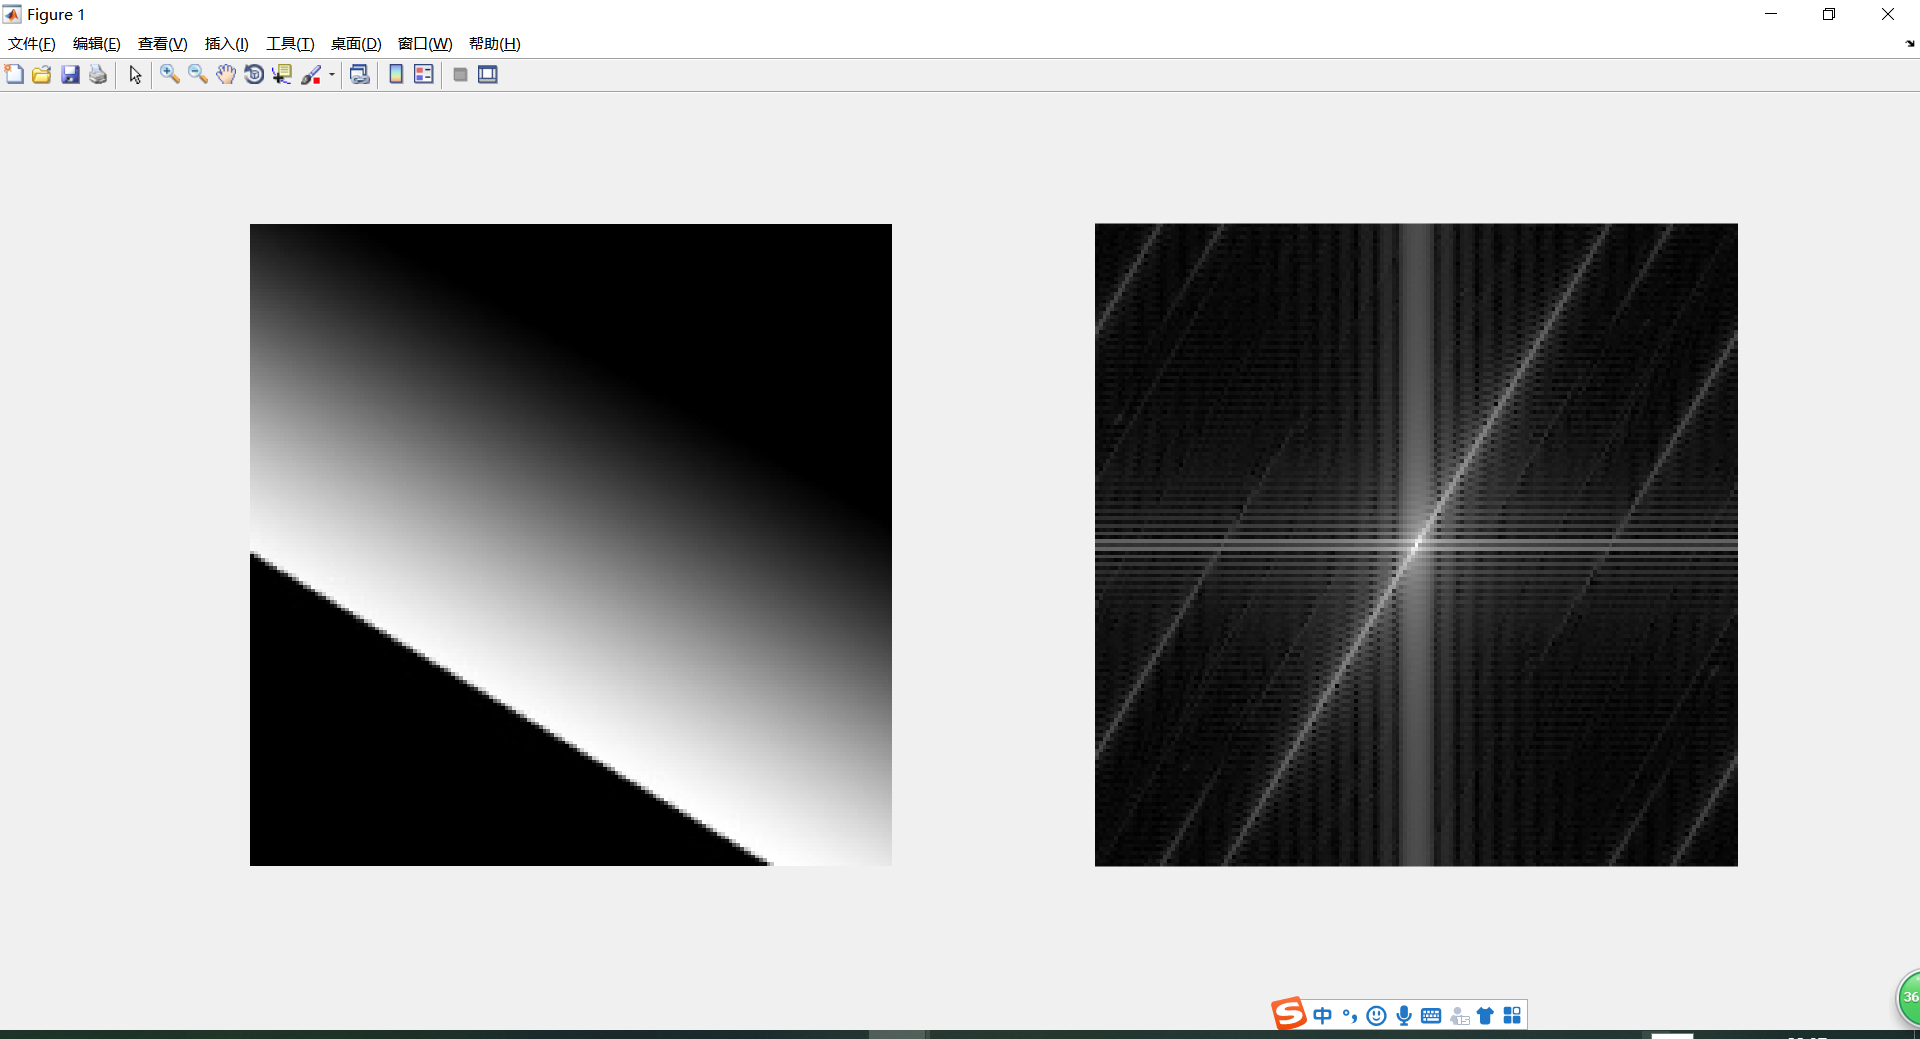
\includegraphics[scale=0.4]{result.png} 
%            	\caption{实验结果} 
%            	\label{result}
%            \end{figure}

            


	\section{总结}
  
        \indent 灰度形态学操作的数学表达式比较复杂,不太容易理解,所以本次报告重点从几何的角度用语言来描述四种操作。
        
        \indent 从性能上来说,形态学有着坚实的数学理论支撑,同时操作简单,计算复杂度低,相比之前的各种滤波操作,在很多情况下形态学操作有着难以替代的优势,是提取图像特征,如边界、骨架、凸壳等的有力工具。
%			\begin{figure}[H]
%				\centering 
%				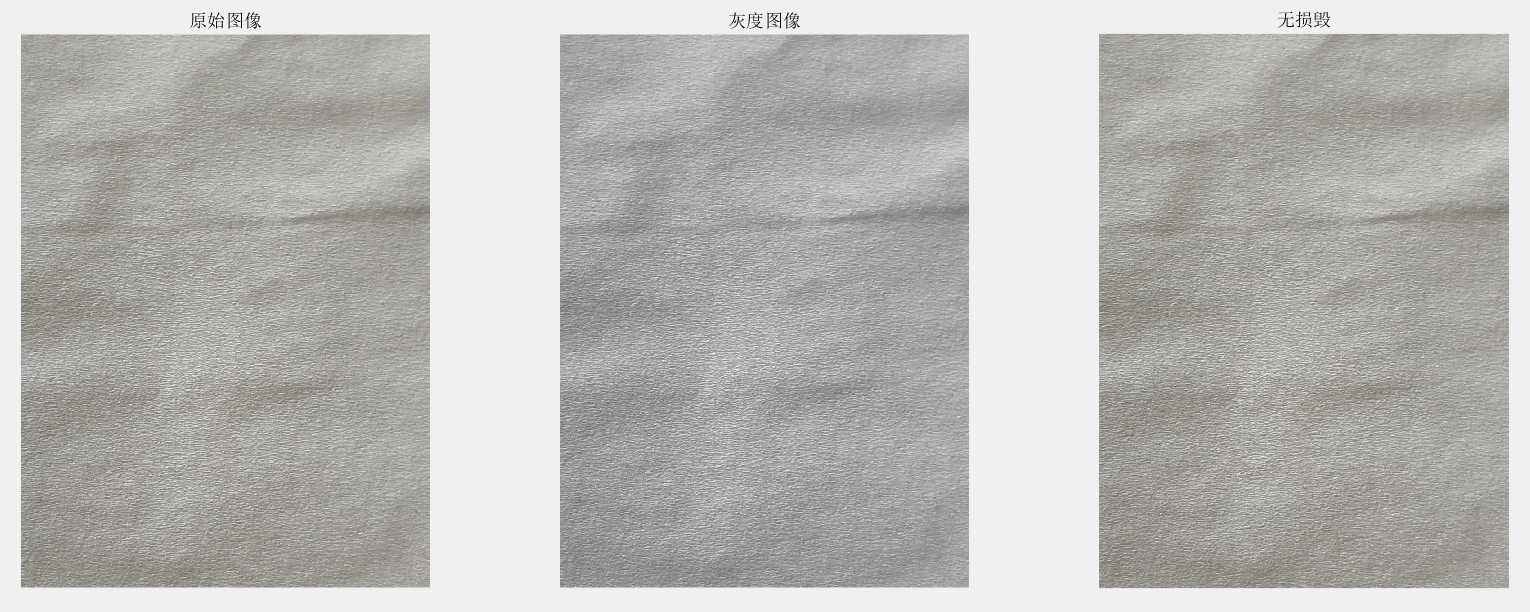
\includegraphics[scale=0.4]{res4.png} 
%				\caption{结果4} 
%				\label{res4}
%			\end{figure}
		

		
%			\begin{figure}[H]
%				\centering 
%				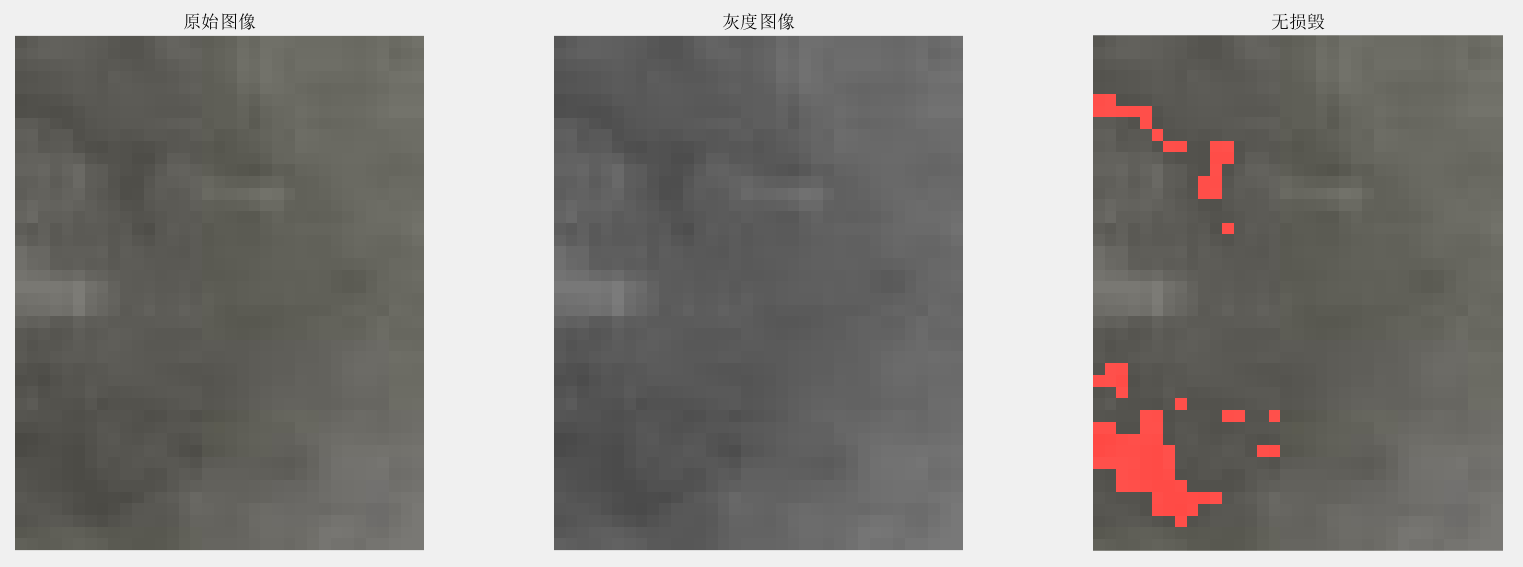
\includegraphics[scale=0.4]{res6.png} 
%				\caption{结果6(截取自结果5的阴影部分)} 
%				\label{res6}
%			\end{figure}
	
	
% 中文文献多个作者用中文逗号“,”连接
%\bibliography{ref.bib}
%\bibliographystyle{abbrv}
\bibliography{ref.bib}


\end{document}